\subsection{WSML Semantics through Meta-Level Axioms}
%-- describe how a fixed set of rules implements (part of) the WSML semantics during reasoning \\
%-- -- each WSMl entity is mapped to a datalog constant \\
%-- -- special meta-level predicates stand for specific WSMl constructs with a certain semantics; they are applied to datalog constants (give example in picture) \\
%-- -- a direct mapping would not facilitate metamodelling as a feature of WSML \\
%-- -- meta-level axioms assure that the proper semantics of the wSMl constructs is maintained \\
%-- -- the meta-level axioms form rules for the meta-level predicates (, which appear in these rules) \\
%-- -- explain the intuition behind the various meta-level axioms \\

The mapping from WSML to datalog in the reasoning framework works
such that each WSML-identifiable entity, i.e.\ concept, instance,
attribute etc., is mapped to an instance (or logical constant) in
datalog, as depicted in Figure \ref{fig:meta}. There, the concepts
$C_1, C_2, C_3$ as well as the instances $I_1, I_2$ and the
attribute $a$ are mapped to constants such as $I_{C_1}$, $I_{I_1}$
or $I_a$ in datalog, representing the original WSML entities on
the instance level.

Accordingly, the various special-purpose relations that hold
between WSML entities, such as \wsml{subConceptOf},
\wsml{memberOf} or \wsml{hasValue}, are mapped to datalog
predicates that form a meta-level vocabulary for the WSML language
constructs. These are the meta-level predicates that appear in
Table \ref{tab:LE2datalog}, and which are applied to the datalog
constants that represent the WSML entities. The facts listed in
Figure \ref{fig:meta} illustrate the use of the meta-level
predicates. For example, the predicate \psco takes two datalog
constants as arguments that represent WSML concepts, to state that
the concept represented by the first argument is a subconcept of
the one represented by the second argument; on the other hand, the
predicate \pmo takes a datalog constant that represents a WSML
instance and one that represents a WSML concept, to state that the
instance is in the extension of this concept.

In contrast to a direct mapping from WSML to datalog with
concepts, attributes and instances mapping to unary predicates,
binary predicates and constants, respectively, this indirect
mapping allows for the WSML metamodelling facilities.
Metamodelling allows an entity to be a concept and an instance at
the same time. By representing a WSML entity as a datalog
constant, it could, for example, fill both the first as well as
the second argument of e.g.\ the predicate \pmo, in which case it
is interpreted as both an instance and a concept.

\begin{figure}[tb]
        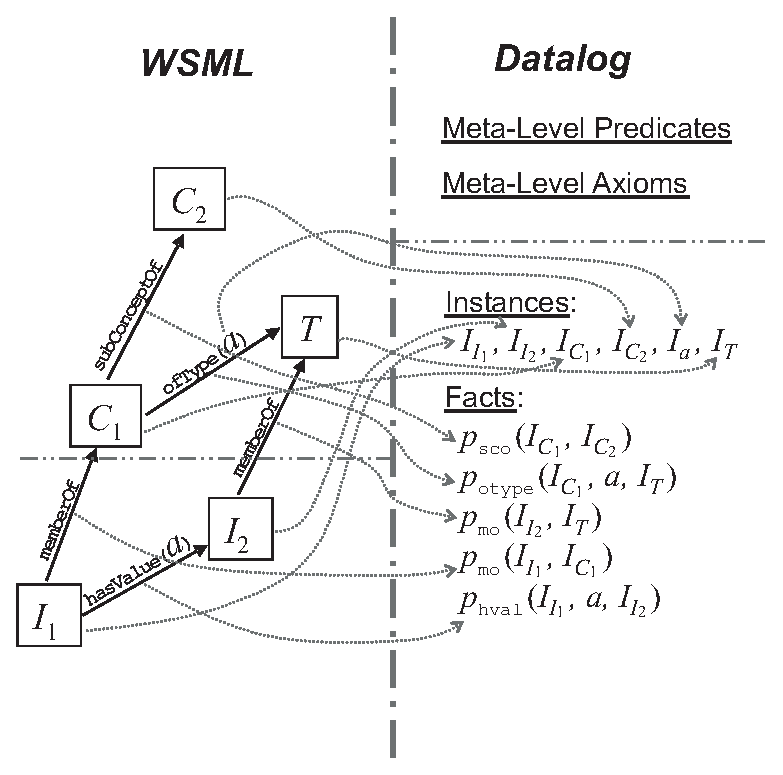
\includegraphics[width=8cm]{figures/meta}
        \centering
    \caption{Usage of meta-level predicates. \label{fig:meta}}
\end{figure}

% -- old table for meta-level predicates + meta-level axioms
%\def\filler{\phantom{l}}
%\begin{table}[tb]\label{tab:meta-level}\centering
%\begin{tabular}{|l|l|}
%  \hline
%  \multicolumn{2}{|l|}{\emph{Meta-Level Predicates}} \\
%  \filler \begin{small}Predicate\end{small} & \begin{small}WSML construct\end{small} \\
%  \hline
%  \filler $\psco(C_{sub},C_{sup})$ \qquad\qquad & $C_{sub}$ \wsml{subConceptOf} $C_{sup}$ \\
%  \filler $\pmo(I,C)$ & $I$ \wsml{memberOf} $C$ \\
%  \filler $\phval(I,a,V)$ & $I[a$ \wsml{hasValue} $V]$ \\
%  \filler $\pitype(C,a,T)$ & $C[a$ \wsml{impliesType} $T]$ \\
%  \filler $\potype(C,a,T)$ & $C[a$ \wsml{ofType} $T]$ \\
%  \hline\hline
%  \multicolumn{2}{|l|}{\emph{Meta-Level Axioms}} \\
%  \hline
%  \multicolumn{2}{|l|}{\filler $\psco(C_1,C_3) \leftarrow \psco(C_1,C_2) \wedge \psco(C_2,C_3)$} \\
%  \multicolumn{2}{|l|}{\filler $\pmo(I,C_2) \leftarrow \pmo(I,C_1) \wedge \psco(C_1,C_2)$} \\
%%  \multicolumn{2}{|l|}{\filler $\pmo(V,C_2) \leftarrow \pitype(C_1,a,C_2) \wedge \pmo(I,C_1) \wedge \phval(I,a,V)$} \\
%  \multicolumn{2}{|l|}{\filler $\pmo(V,C_2) \leftarrow \pitype(C_1,a,C_2) \wedge \pmo(I,C_1)$} \\
%  \multicolumn{2}{|l|}{\filler \phantom{$\pmo(V,C_2) \leftarrow$} \qquad $\wedge \phval(I,a,V)$} \\
%%  \multicolumn{2}{|l|}{\filler $ \leftarrow \potype(C_1,a,C_2) \wedge \pmo(I,C_1) \wedge \phval(I,a,V) \wedge \neg \pmo(V,C_2)$} \\
%  \multicolumn{2}{|l|}{\filler $ \leftarrow \potype(C_1,a,C_2) \wedge \pmo(I,C_1)$} \\
%  \multicolumn{2}{|l|}{\filler $ \phantom{\leftarrow} \qquad \wedge \phval(I,a,V) \wedge \neg \pmo(V,C_2)$} \\
% \hline
%\end{tabular}
%\caption{Meta-level axioms and predicates for WSML semantics in
%datalog.}
%\end{table}
\begin{table}[tb]\label{tab:meta-level}\centering
\begin{small}
\begin{tabular}{|ll|}
  \hline
  \multicolumn{2}{|l|}{\rule{0cm}{3.2mm}{\normalsize \emph{Meta-Level Axioms}}} \\
  \hline
  (1) & $\psco(C_1,C_3) \dlogrule \psco(C_1,C_2) \dlogand \psco(C_2,C_3)$ \\
  (2) & $\pmo(I,C_2) \dlogrule \pmo(I,C_1) \dlogand \psco(C_1,C_2)$ \\
  (3) & $\pmo(V,C_2) \dlogrule \pitype(C_1,a,C_2) \dlogand \pmo(I,C_1)$ \\
  & \phantom{$\pmo(V,C_2) \dlogrule$} $\dlogand \phval(I,a,V)$ \\
  (4) & $\dlogcstr \potype(C_1,a,C_2) \dlogand \pmo(I,C_1)$ \\
  & \phantom{$\dlogcstr$} $\dlogand \phval(I,a,V) \dlogand \dlognot \pmo(V,C_2)$ \\
 \hline
\end{tabular}
\end{small} \caption{Realising WSML semantics in
Datalog.}
\end{table}

A fixed set \mlaxioms of datalog rules forms the meta-level axioms
which assure that the proper semantics of the WSML language is
maintained. In these axioms, the meta-level predicates are
interrelated according to the semantics of the different language
constructs. Table \ref{tab:meta-level} shows the rules that make
up the meta-level axioms in \mlaxioms. Axiom (1) realizes
transitivity for the WSML \wsml{subConceptOf} construct, while
axiom (2) ensures that an instance of a subconcept is also an
instance of its superconcepts. Axiom (3) realizes the semantics
for the \wsml{implisType} construct for attribute ranges: any
attribute value is concluded to be in the extension of the range
type declared for the attribute. Finally, axiom (4) realizes the
semantics of the \wsml{ofType} construct by a constraint that is
violated whenever an attribute value cannot be concluded to be in
the extension of the declared range type.
